% Created 2017-04-05 Wed 11:04
% Intended LaTeX compiler: pdflatex
\documentclass[10pt,oneside,x11names]{article}
\usepackage[utf8]{inputenc}
\usepackage[T1]{fontenc}
\usepackage{graphicx}
\usepackage{grffile}
\usepackage{longtable}
\usepackage{wrapfig}
\usepackage{rotating}
\usepackage[normalem]{ulem}
\usepackage{amsmath}
\usepackage{textcomp}
\usepackage{amssymb}
\usepackage{capt-of}
\usepackage{hyperref}
\usepackage{geometry}
\usepackage{amsmath}
\usepackage{amssymb}
\usepackage{amsfonts}
\usepackage{palatino}
\usepackage{siunitx}
\usepackage{esdiff}
\usepackage{xfrac}
\usepackage{nicefrac}
\usepackage{faktor}
\usepackage[euler-digits,euler-hat-accent]{eulervm}
\author{Brian Beckman}
\date{\textit{<2017-04-05 Wed>}}
\title{Junior Johnson vs. the Dwarves}
\hypersetup{
 pdfauthor={Brian Beckman},
 pdftitle={Junior Johnson vs. the Dwarves},
 pdfkeywords={},
 pdfsubject={},
 pdfcreator={Emacs 25.1.1 (Org mode 9.0.5)}, 
 pdflang={English}}
\begin{document}

\maketitle
\setcounter{tocdepth}{2}
\tableofcontents


\section{}
\label{sec:orgb999c5b}
\begin{center}
\includegraphics[width=.9\linewidth]{./junior_johnson_3.jpg}
\end{center}\begin{center}

\includegraphics[width=.9\linewidth]{./hqdefault.jpg}
\end{center}
\section{Deliver the Hooch!}
\label{sec:org65306d3}
\subsection{Deadline! Drive Like Junior Johnson}
\label{sec:orgea489f7}
\subsubsection{100 mph in the woods at night with the headlights off}
\label{sec:org72c08bd}
\begin{center}
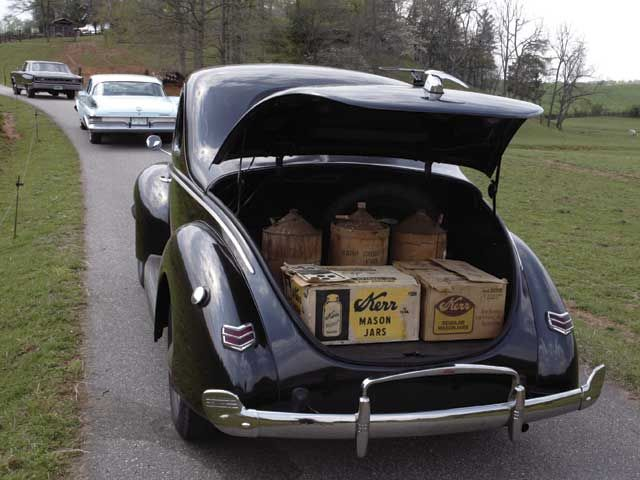
\includegraphics[width=.9\linewidth]{./6a00d8341bfe8453ef0134802e46f2970c-800wi.hooch.jpg}
\end{center}
\subsection{Gotta be lucky AND good}
\label{sec:org38fab8d}
\subsubsection{hit a tree? you have a problem}
\label{sec:orgcce4ad6}
\subsubsection{no telling how long till you're going again}
\label{sec:org863556b}
\subsubsection{you might not make it}
\label{sec:org0be90b7}
\section{Choice 2: Dig a Tunnel}
\label{sec:org7d64b02}
\begin{center}
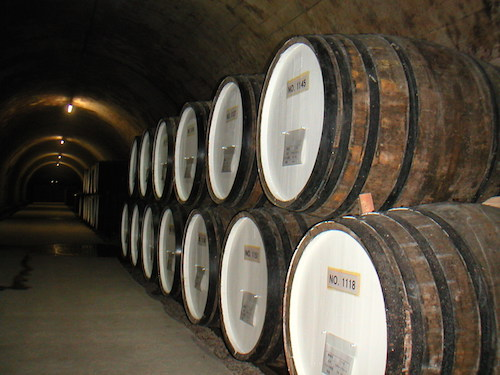
\includegraphics[width=.9\linewidth]{./whiskey_tunnel_desc01.jpg}
\end{center}
\subsection{You only have to be good}
\label{sec:orgac5c026}
\subsubsection{takes longer, but no backtracking and search / debugging}
\label{sec:orgbb56ab5}
\begin{enumerate}
\item time is more predictable
\label{sec:org70a5a94}
\end{enumerate}
\subsubsection{lots of time for certification, documentation, proofs (``high assurance'')}
\label{sec:org89bdb78}

\section{Summary \& Disclaimer}
\label{sec:org7a1214c}
\subsection{WIP: Not fully thought out}
\label{sec:orge1fc041}
\subsubsection{I reserve the right to change my mind}
\label{sec:org34b18df}
\subsubsection{TDD ``feels'' better because it sidesteps debugging}
\label{sec:orgfb26e81}
\begin{enumerate}
\item Makes every programming language feel like a REPL
\label{sec:orge0a93cd}
\item Unpredictable debugging pitfalls are avoided more frequently
\label{sec:org5bcd0cb}
\item Easily defensible for exploratory designs
\label{sec:org2a47bee}
\item Defensible when large test corpora are required for certification
\label{sec:org436dd95}
\item Less defensible under time pressure
\label{sec:org97f1b75}
\end{enumerate}
\subsubsection{Irony: defensible at the extremes of development}
\label{sec:orgb6e77c1}
\begin{enumerate}
\item When you're not sure what you're doing (``science'')
\label{sec:org9b3bdae}
\item When you're absolutely sure what you're doing (``engineering with high QA'')
\label{sec:org8bded85}
\end{enumerate}
\subsubsection{I have VERY recent experiences to talk about}
\label{sec:orga989fda}
\subsection{As Always: ``Unless You Know Better''}
\label{sec:orga992582}
\section{A Story}
\label{sec:org97bbe2f}
\subsection{I'm digging along}
\label{sec:org0559943}
\subsubsection{on schedule to deliver certifiable nav filter in three weeks}
\label{sec:orgdcda1c9}
\subsubsection{phone call! ``We're flying Wednesday! Deliver MONDAY!}
\label{sec:orgff1ad55}
\section{A Story}
\label{sec:org05b5015}
\subsection{Tuesday Night, slam-coding basics from a paper}
\label{sec:org22d2b83}
\(B=\begin{cases} \begin{matrix} \frac { 1 }{ 2 } -\frac { \theta ^{ 2 } }{ 4! }
+\frac { \theta ^{ 4 } }{ 6! } , & | \theta | \, \lesssim \, 10^{ -7 } \end{matrix}
\\ \begin{matrix} { \left( 1-\cos { \theta  }  \right)  }/{ { \theta  }^{ 2 } }
& \mathrm{otherwise} \quad  \end{matrix} \end{cases}\)

if (std::abs(th) < SMALL\(_{\text{ANGLE}}\)) \{
    B = (0.5 - th * th * 1.0 / 24.0
\begin{itemize}
\item th * th * th * th * 1.0 / 720.0);
\end{itemize}
\} else \{ B = (1.0 - cos(th)) / th * th; \}

\section{A Story}
\label{sec:orge656132}
\subsection{Wednesday --> Friday, Three Thousand More Lines}
\label{sec:orgfbf8ea6}
\subsection{Friday Night, Integration Time, Something is Wrong}
\label{sec:orgeb63967}
\subsubsection{Can you finish by Monday?}
\label{sec:orge021dd7}

\section{A Story}
\label{sec:orgc373ee2}
\(x/yz\)
\subsubsection{``the manuscript-submission instructions for the Physical Review journals}
\label{sec:org4b609e5}
\subsubsection{state that multiplication is of higher precedence than division with a slash,}
\label{sec:org99ebeec}
\subsubsection{and this is also the convention observed in prominent physics textbooks such}
\label{sec:org3664c2d}
\subsubsection{as the Course of Theoretical Physics by Landau and Lifshitz and the}
\label{sec:org739c784}
\subsubsection{Feynman Lectures on Physics.``}
\label{sec:orge6547c2}
\subsubsection{What does it mean?}
\label{sec:org374770c}
\subsubsection{``the manuscript-submission instructions for the Physical Review journals  \ldots{}}
\label{sec:orgfadc813}
\subsection{But C / C++ / Python / MATLAB / etc. say}
\label{sec:org6eba29f}
\(x/yz = xz/y\)
\subsection{Unit Testing would have caught this Tuesday}
\label{sec:orgc5bb799}
\subsection{Putting off testing to Friday requires us to debug / search}
\label{sec:orgeacaf70}
\subsubsection{Actually, this bug was also lurking in MATLAB code transcribed from the same source}
\label{sec:orgea45ae8}

\section{The Tradeoff}
\label{sec:orgc119f70}
\subsection{If you don't need predictable schedule and high assurance}
\label{sec:orgc00a3da}
\subsubsection{You can afford the cost of mistakes}
\label{sec:org361dc2e}
\subsubsection{You can afford occasional missed deadlines}
\label{sec:org964b8e0}
\begin{enumerate}
\item You can afford unbounded debugging time
\label{sec:orge19fef5}
\begin{itemize}
\item Drive Like Junior Johnson
\end{itemize}
\end{enumerate}
\subsection{Otherwise, you need predictable schedule or high assurance}
\label{sec:org74da424}
\subsubsection{You can't afford mistakes (aviation, CPUs, OSs, platform games)}
\label{sec:org6b3ba30}
\subsubsection{You can't afford missed deadlines (contracts, FAA, law suits, jail)}
\label{sec:orgaa33704}
\subsubsection{You can't afford debugging time (channels are backing up)}
\label{sec:org171dc75}
\begin{itemize}
\item Dig a Tunnel: Test-Driven Development (TDD)
\end{itemize}
\section{The Tradeoff}
\label{sec:org98e6430}
\subsection{TDD trades O(N) dev time for O(N log N) debugging time}
\label{sec:orgea5ea9a}
\subsection{Debugging is SEARCH}
\label{sec:orge0bed51}
\subsubsection{The more you write before you test\ldots{}}
\label{sec:org4d22474}
\begin{enumerate}
\item the bigger your search space
\label{sec:orge66f701}
\item time is unpredictable
\label{sec:orgb344393}
\begin{enumerate}
\item but only logarithmically if you're good
\label{sec:orge9f925f}
\end{enumerate}
\end{enumerate}
\subsection{TDD is LINEAR}
\label{sec:orgea95427}
\subsubsection{Tests = Specs = Docs <= Assured Code all at once}
\label{sec:org5ab7370}
\subsubsection{Certification = formalized traceability}
\label{sec:orga116dd8}
\begin{enumerate}
\item Req'ts -> Designs -> Tests
\label{sec:org69a1cce}
\end{enumerate}
\subsubsection{Required by FAA etc.}
\label{sec:orga7dea04}
\section{Unit Tests vs. PBT (Property-Based Testing)}
\label{sec:org406477c}
\subsection{Unit Tests}
\label{sec:org388605c}
\subsubsection{based on examples ``points'' invented by programmers}
\label{sec:orga11cb86}
\subsubsection{limited by the ability of programmers to invent examples that exercise everything pertinent to a spec.}
\label{sec:org076ab6b}
\subsection{Property-Based Testing (PBT)}
\label{sec:orgf346470}
\subsubsection{AKA QuickCheck, hypothesis (Python), rapidcheck (C++), test.check (Clojure)}
\label{sec:orgef2275d}
\subsubsection{generates broader tests, statistically sampling the input domains}
\label{sec:org71336df}
\subsubsection{checks assertions about properties of outputs}
\label{sec:org6284c8b}
\subsubsection{best for comparing independent alternative implementations}
\label{sec:org74ba032}
\subsubsection{limited by the ability of programmers to understand broader, non-obvious properties}
\label{sec:orgbec8507}
\section{Examples:}
\label{sec:org9ac94f5}
\subsection{Kalman Filter in C / C++ / Python}
\label{sec:org08e8093}
\subsection{An Interview Question}
\label{sec:org8aa6c62}
\subsection{Time Warp Operating System}
\label{sec:org88dc679}
\section{Abstract:}
\label{sec:org5e76212}
\subsection{Test-Driven Development (TDD) can deliver higher-quality results with documentation}
\label{sec:org0f25268}
\subsection{and more predictable schedules than can slam-coding and debugging, but it can take longer.}
\label{sec:orgec34d21}
\subsection{It's like digging a tunnel to deliver the moonshine versus driving at 100 mph through}
\label{sec:org88191e0}
\subsection{the woods at night with the headlights off. We present tradeoff analysis and examples}
\label{sec:orge49c3f8}
\subsection{from embedded aviation code in C / C++, where certification authorities often require}
\label{sec:orgb97fa4e}
\subsection{traceable documentation and high assurance (machine-checked coding standards; proofs;}
\label{sec:orgaf61aa1}
\subsection{exhaustive or statistical unit testing; more). We also present examples in Clojure, which}
\label{sec:orgdd07adf}
\subsection{facilitates lightweight formal specs and generative testing for JVM code.}
\label{sec:org11d8af1}

\subsection{Normal unit testing is based on point-like examples invented by programmers (one point}
\label{sec:orgff6fb0b}
\subsection{in input domain mapped to one point in the output range). It's limited by the ability of}
\label{sec:orga5f8a05}
\subsection{programmers to invent examples that exercise everything pertinent to a spec.}
\label{sec:orga46a19a}
\subsection{Property-based testing generates broader tests, statistically sampling the input domains}
\label{sec:org4cc8068}
\subsection{and checking assertions about properties of outputs. It's limited by the ability of}
\label{sec:org8997bf7}
\subsection{programmers to understand broader properties and to imagine non-obvious tests.}
\label{sec:org34cc854}
\end{document}